\section{Problem Formulation\label{sec:ch8:formulation}}

In this section, the problem formulation for the combined architecture, plant, and control design of a quarter-car vehicle suspension is described.

%--------------------------------------
\subsection{Architecture Specification}

\begin{figure}
\centering
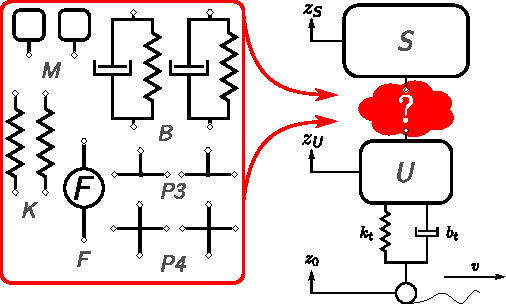
\includegraphics[width=0.55\columnwidth]{../ch8/figures/suspension1}
\caption{Suspension architecture component catalog.\label{fig:ch8:suspension1}}
\end{figure}

The component catalog and NSCs will be the same as the case study in Sec.~\ref{sec:ch2:example4}.
The $(\gls{C}, \gls{R}, \gls{P})$ specification is:
\begin{subequations}
\label{eq:ch8:CRP}
\begin{align}
C &= \{\xcolor{S}, \xcolor{U},  \xcolor{M},  \xcolor{K},  \xcolor{B},  \xcolor{F}, \xcolor{P3}, \xcolor{P4} \} \\
R &= \begin{bmatrix} 1,1,2,2,2,1,2,2 \end{bmatrix} \\
P &= \begin{bmatrix} 1,1,1,2,2,2,3,4 \end{bmatrix}
\end{align}
\end{subequations}

\noindent The catalog is represented in Fig.~\ref{fig:ch8:suspension1}.
Each of the component types fits in the bond graph modeling paradigm: $\{\xcolor{S}, \xcolor{U},  \xcolor{M}\}$ are \xcolor{I}-type storage nodes, \xcolor{K} is a \xcolor{C}-type storage node, \xcolor{B} is a subsystem containing a spring and damper in parallel (see Fig.~\ref{fig:ch8:suspension1}), and \xcolor{F} is an \xcolor{Se}-type effort source.
The remaining component types represent \xcolor{1}-junctions with a differing connection numbers.

% new paragraph
The architecture-only objective function term is the sum of the additional physical components (i.e.,~everything but \xcolor{S}, \xcolor{U}, and \xcolor{P}$x$):
\begin{align}
\Psi_a = \gls{weights}_a\left( \gls{number}_{\xcolor{M}} + n_{\xcolor{K}} + n_{\xcolor{B}} + n_{\xcolor{F}} \right)
\end{align}

\noindent where $w_a$ is the weighting coefficient.
This just one metric for complexity that we can use to look at tradeoffs between complexity and performance.

%--------------------------------------
\subsection{Co-Design Problem}

Three outputs will be needed to capture the co-design problem formulation:
\begin{align}
\bm{y} = \begin{bmatrix} z_{\xcolor{U}} \\ \ddot{z}_\xcolor{S} \\ z_\xcolor{S} \\ u \end{bmatrix}
\end{align}

\begin{subequations}
\noindent namely the unsprung mass position, sprung mass acceleration, unsprung mass position, and control.
The co-design objective function is the sum of several performance metrics:
\begin{align} \label{eq:ch8:susobj}
\Psi_d = \int_{t_0}^{t_f} \left( w_1 \left( y_1 - z_0 \right)^2 + w_2 y_2^2 + w_3 y_4^2 \right) dt
\end{align}

\noindent where the term $w_1 \left( y_1 - z_0 \right)^2$ captures the handling objective, $w_2 y_2^2$ represents the passenger comfort objective, and $w_3 y_4^2$ control effort objective (see Refs.~\cite{Allison2014b, Alyaqout2007b, Fathy2003a}).

% new paragraph
Next, the states of the system are initialized to their zero equilibrium position with the following simple bound constraint: 
\begin{align}
\bm{\xi}\xarch(t_0) = \bm{0} 
\end{align}

To ensure that the separation between the sprung and unsprung masses remains tolerable, the following rattlespace constraint is necessary \cite{Allison2014b, Fathy2003a, Gobbi2001a, Hrovat1993a, Ulsoy1994a}:
\begin{align}
\abs{y_3 - y_1} \leq \gls{rattlespace}
\end{align}

\noindent This constraint can be converted into two linear constraints as is shown in Sec.~\ref{sec:ch5:absolute:values}.
The rattlespace constraint is commonly included in the objective function but is more appropriately included as a constraint.
The LQDO problem class can readily handle linear inequality constraints unlike other solution strategies \cite{Allison2014b,manuscript-dt-qp}.

% new paragraph
All the previous constraints are necessary for the inner-loop co-design problem.
The outer-loop specific plant constraints are simple bounds on the linear coefficients:
\begin{align}
\gls{mass}_{\glsfoo[noindex]{min}} \leq \bm{x}_m\xarch \leq m_{\glsfoo[noindex]{max}} \\
\gls{damper}_{\min} \leq \bm{x}_b\xarch \leq b_{\max} \\
\gls{spring}_{\min} \leq \bm{x}_k\xarch \leq k_{\max} 
\end{align}

\noindent where the subscripts $\{m,b,k\}$ indicate the additional mass, damper, and spring plant variables for the candidate architecture.

\end{subequations}

\begin{table}
\centering
\begin{tabular}{cc|cc}
\hline \hline
Parameter & Value & Parameter & Value \\
\hline
$w_1$ & $10^5$ & $k_t$ & $232\times 10^3$ N/m \\
$w_2$ & $0.5$ & $b_t$ & $0$ Ns/m \\
$w_3$ & $10^{-5}$ & $r_{\max}$ & $0.03$ m \\
$t_0$ & $0$ s & $t_f$ & $9$ s \\
$m_{\min}$ & $0.001$ kg & $m_{\max}$ & $5$ kg  \\
$b_{\min}$ & $10^3$ Ns/m & $b_{\max}$ & $10^6$ Ns/m \\
$k_{\min}$ & $10^3$ N/m & $k_{\max}$ & $10^7$ N/m \\
$m_{\xcolor{U}}$ & $65$ kg & $m_{\xcolor{S}}$ & $325$ kg \\
\hline \hline
\end{tabular}
\caption{Co-design problem parameters.\label{tb:ch8:parameters}}
\end{table}

The problem parameters used in this study are shown in Table~\ref{tb:ch8:parameters} (many of the parameters are based the study in Ref.~\cite{Allison2014b}).
A rough road input is used from Refs.~\cite{Allison2008b, Allison2014b}.